%!TEX root = Journal.tex
In this section, the transmission model described in Section~\ref{sec:Model} is applied to the IEEE 30-bus system, shown in Fig.
\ref{fig:wee}. Interested readers are referred to \cite{zimmerman2009matpower} for
detailed parameters of the TS. The MG export cost $c^{ex}_{t}$ is defined to be $0.9*c^{im}_{t}$. The parameters of the 25 MW MG is listed in the appendix.  Multiple wind farms are positioned at different buses in the TS to provide renewable generation. A comprehensive MG is considered in this work. The MG consists of a
generator, a storage unit, DL and non-DL, and is able
to operate in islanded mode and grid-connected mode. The parameter values of the 25 MW MG are listed in the appendix.
\begin{figure}[H]
\centering
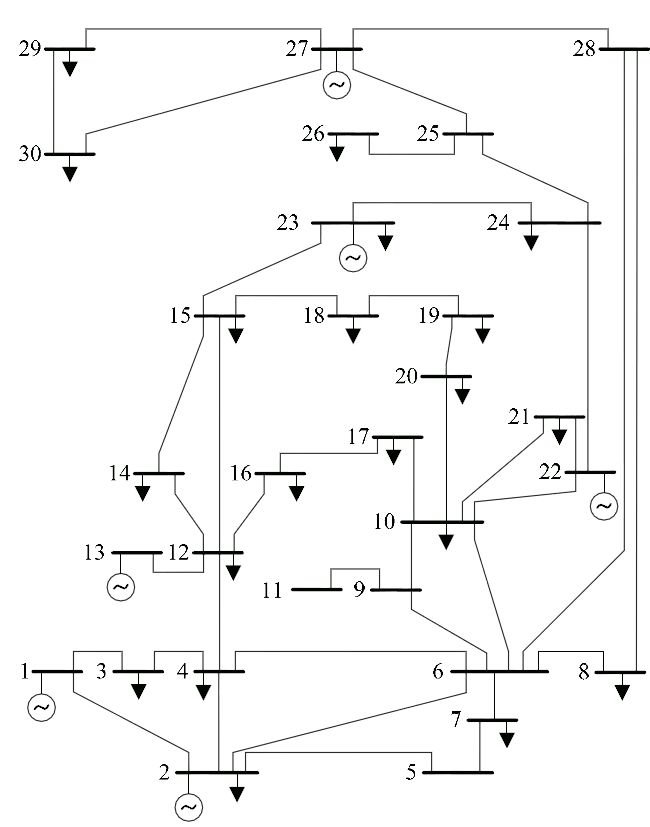
\includegraphics[scale=0.4]{IEEE_30bus.png}
\caption{IEEE 30 Bus System}
\label{fig:wee}
\end{figure}

The wind data for the wind farms in the TS are selected from the
NREL-Eastern Wind Integration Study dataset \cite{energy2010eastern}.
Using three years of data, 24-hour trajectories are grouped
to identify a set of 54 similar trajectories, with a common initial
condition. The set of trajectories was used
to represent the realizations of a similar forecast. The central
trajectory of the group was selected as the wind forecast,
and the remaining were used to estimate the distribution of
forecast errors, as described in \cite{anderson2011wind}. From the forecast error
distribution, 10000 scenarios are used to generate a robust
wind error scenario set. 

%For the MG import price, the locational marginal price for each buse in the TS without the MG is precomputed for a wide range of loading conditions. Then a first order equation is fitted between the price and the import quantity. This way the import price is approximated as a linear function of the import quantity as below:
%\begin{subequations}
%\begin{align}
%C^{im}_t = a*P^{im}_t + b
%\end{align}
%\end{subequations}
%where $a$ and $b$ are two constants representing the slope and intercept of the pricing equation. The method enables a dynamic pricing scheme which accounts for varying system loading conditions and at the same time preserves the convexity of the problem. The export price is defined as 90\% of the import price at each quantity to avoid the market flaw of buying energy and selling back to make money. This pricing scheme might not be the best pricing scheme. The optimal pricing scheme is out of the focus and scope of the work.

The objective of this work is to analyze different factors that affect the WP in the TS and the operational cost of the two systems in this co-optimization framework as well as the standalone framework. To this end, this section is divided into a WP result part and system cost part.
\subsection{WP Results}

The definition of WP is based on the wind power capacity penetration defined by the European Wind Energy Association \cite{european2012wind}. It is the ratio of the installed wind capacity divided by the peak system load.

\subsubsection{Location of Wind in the System}
To generate some benchmarks, a wind farm is positioned at different buses in the TS with no MG. The maximum WP in each case is recorded. The results for some representative bus are given in Table\ref{transbus}.

\begin{table}[H]
\centering
\begin{tabular}{ |c|c|c| } 
 \hline
 Wind Bus & Max WP & Reason \\ 
 \hline
5 & 38\% & Use up generator reserve \\ 
 \hline
8 & 28\% & Reach transmission limit\\ 
 \hline
15 & 38\% & Use up generator reserve \\ 
 \hline
30 & 28\% & Reach transmission limit \\ 
 \hline
8 and 30 & 38\% & Use up generator reserve \\ 
 \hline
\end{tabular}
\caption{ WP at different buses}
 \label{transbus}
\end{table}

As the TS has a network with limits on transmission lines, different buses have different capacities in terms of renewable injection. Table \ref{transbus} shows that bus 8 and 30 allows smaller WPs compared to bus 5 and 15 as bus 8 and 30 are connected to transmission lines with smaller capacity. For bus 5 and 15, the connected line capacity is large enough to use up the generator reserve to achieve maximum WP. When there are two wind farms at bus 8 and 30, all the generator reserve is used to account for the wind forecast deviation as the combined line capacity at those two buses is large enough to use up the generator reserve. Therefore, wind farms should avoid buses with tight transmission constraints in terms of their placement. The method to find buses that are more prone to violate transmission constraints in given in \cite{liu2016quantifying}. As a result, wind farms should be placed at buses with generous transmission capacity and possibly at multiple locations to achieve high level of WP.

\subsubsection{WP with a MG}
To illustrate the effects of MG on the WP, a 25MW MG with 50\% DL is connected to the wind buses in the previous section. Here the DL percentage is defined as the ratio of the maximum DL and the sum of maximum DL and non-DL. The size of the MG (25MW in this case) is defined as the generation capacity of the MG. The WP with and without the MG is given in Fig.\ref{fig:wp}.

\begin{figure}[H]
\centering
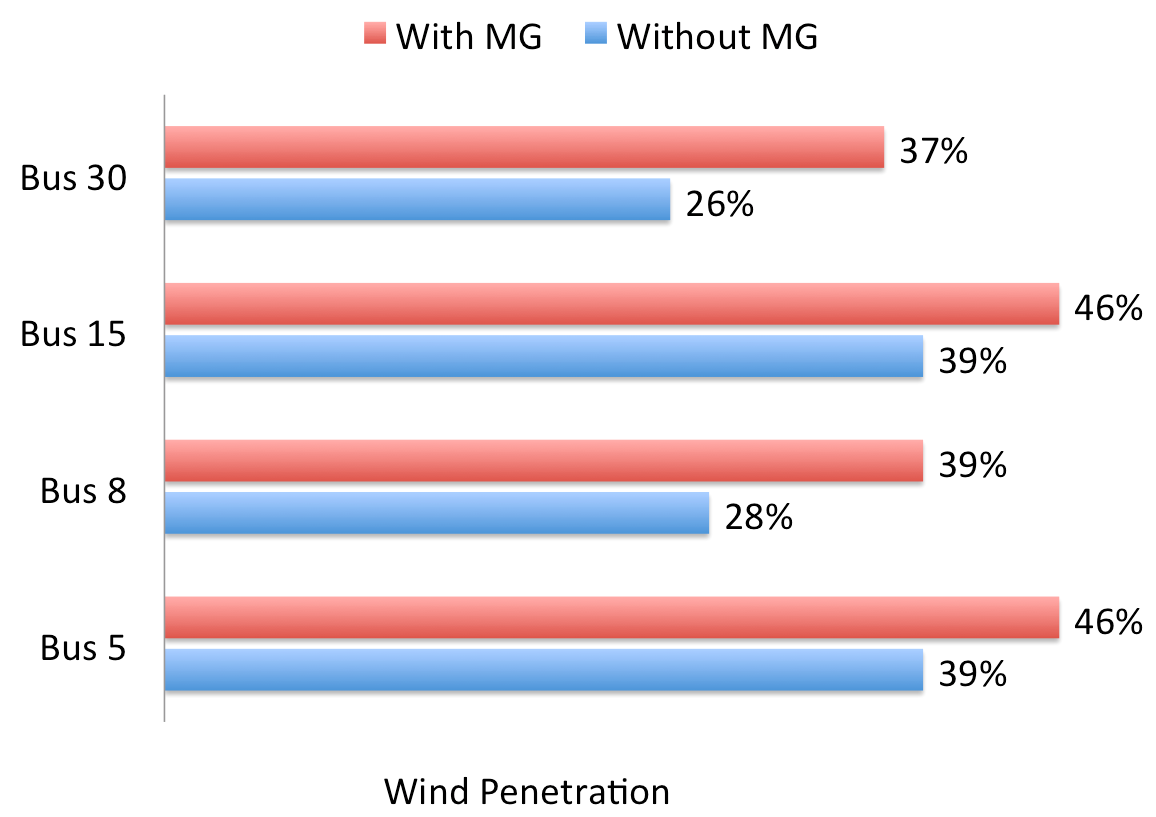
\includegraphics[scale=0.25]{windp.png}
\caption{WP with and without MG at different buses}
\label{fig:wp}
\end{figure}

Fig.\ref{fig:wp} illustrates that the WP in general increases since the DR provided by the MG could act as reserve and locally offset some wind forecast error at the wind bus. The penetration increase for bus 8 and 30 is more than that of bus 5 and 15 as the MG and TS energy exchange at bus 8 and 30 frees some line capacity for the generator reserves. This case shows that the MG could alleviate congestion under the current energy exchange pricing scheme. This observation is consistent with the results in \cite{liu2016quantifying}. Therefore, for congestion management purpose, MGs should be placed at buses with congestions under this optimization framework.
% and the wind injection consumes some line capacity. 
% Due to power flow constraints, some simulation results show that MG might not always result in an increase in WP as the net injection into the bus could cause congestion and decrease the supply of generator reserve. For example, when the MG and wind farm are both at bus 8 and the MG energy cost is very low for some periods, the MG will export energy into the TS and cause serious congestion, the WP in this case could be equal or even below 28\%. A key lesson from this counter example is that the MG makes decision to maximize its own welfare which might not help with maximizing WP. 
Table \ref{transbuss} shows the the maximum WP when the MG is placed at different buses from the wind farm bus. This table shows that when the MG and wind farm are at different buses, the  WP level could only be less than that when they are at the same bus as the later case could bypass transmission constraints and directly offset wind forecast error, which is not possible for the former case. 

\begin{table}[H]
\centering
\begin{tabular}{ |c|c|c| } 
 \hline
 Wind Bus & MG Bus & Max WP \\ 
 \hline
5 & 8 & 45\% \\ 
 \hline
5 & 15 & 45\% \\ 
 \hline
5 & 30 & 45\% \\ 
 \hline
8 & 5 & 28\%\\ 
 \hline
8 & 15 & 28\% \\ 
 \hline
8 & 30 & 28\% \\ 
 \hline
\end{tabular}
\caption{ WP with the wind farm and MG at different buses}
 \label{transbuss}
\end{table}


%In order to truly achieve the maximum WP that both systems could support, a more sophisticated pricing schemes need to be designed that links the WP to MG's wellfare. However, this is out

%Two typical scenarios that do not result in WP increase is illustrated in Table \ref{noinc}.

%\begin{table}[h]
%\centering
%\begin{tabular}{ |c|c|c| } 
% \hline
% Wind and MG Bus & Scenario & Max WP \\ 
% \hline
%8 & 27\% & Violate transmission limit due to too much energy export from MG  \\ 
% \hline
%30 & 28\% & Violate transmission limit due to too much downward DR \\ 
% \hline
%\end{tabular}
%\caption{ WP at different buses}
% \label{transbus}
%\end{table}

\subsubsection{WP for different MG sizes and DL levels}
As the amount of reserve is proportional to the size of the MG and the amount of DL in the MG, the WP with regards to those two factors are analyzed here. To simulate a MG with varying sizes, the MG parameters except for the ones related to the costs are scaled by the same constant. The wind farm and MG are both located at bus 5 to guarantee enough line capacity and no interference from line constraints. Fig. \ref{wpd} shows WPs for different sizes of a MG with 50\% of the loads being dispachable. Fig. \ref{wpdd} shows WPs for a 25MW MG with different levels of DLs. It can be seen from the two figures that WPs are linearly proportional to MG size and DL levels as there is more MG DR to offset the wind forecast error. 
%However, it is still possible for the MG to cause congestion anomalies at some buses as described in the previous subsection and violate the general rules here.

\begin{figure}[H]
\centering
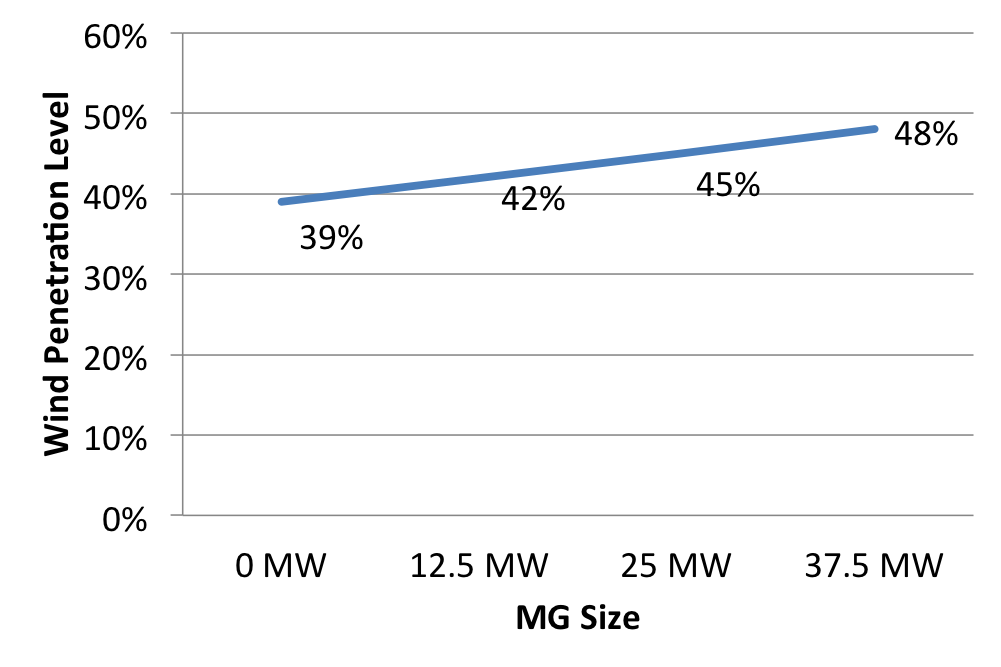
\includegraphics[scale=0.55]{windpd.png}
\caption{WP for different MG sizes}
\label{wpd}
\end{figure}

\begin{figure}[H]
\centering
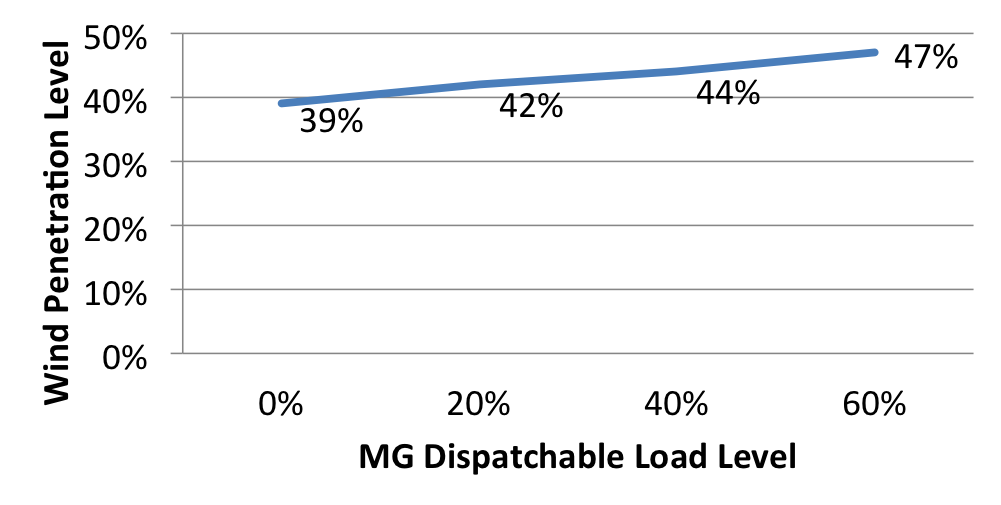
\includegraphics[scale=0.55]{windpdd.png}
\caption{WP for different DL levels}
\label{wpdd}
\end{figure}

\subsection{System Cost Results}
One goal of the TS and MG co-optimization is to reduce the individual system's operation cost. Different factors that affect the cost of the two systems are explored in this section. For the figures in this subsection, SA stands for standalone mode, while COOP stands for co-optimization mode. In the COOP mode, the MG is able to provide DR as reserve to account for the wind forecast error in the TS and exchange energy with the TS. In the SA mode, the MG is separated from the TS and thus could not exchange energy with the TS or provide any DR.

\subsubsection{WP on transmission and MG cost}
As WP is a key concern of the future grid and also a focus of this study, the WP is varied to see the impact on the TS and MG cost. The wind farm and a 25MW MG with 50\% DL is connected to bus 5. The results are displayed in Fig. \ref{pdsize1}.

%\begin{table}[h]
%\centering
%\begin{tabular}{ |c|c|c| } 
% \hline
% WP & Transmission Cost & MG Cost \\ 
% \hline
%0\% & 9068 & 1440  \\ 
% \hline
%5\% & 9095 & 1332 \\ 
% \hline
%10\% & 9376 & 1347 \\ 
% \hline
%15\% & 9682 & 1336 \\ 
% \hline
%\end{tabular}
%\caption{ WP at different buses}
% \label{wdlevel}
%\end{table}
\begin{figure}[H]
\centering
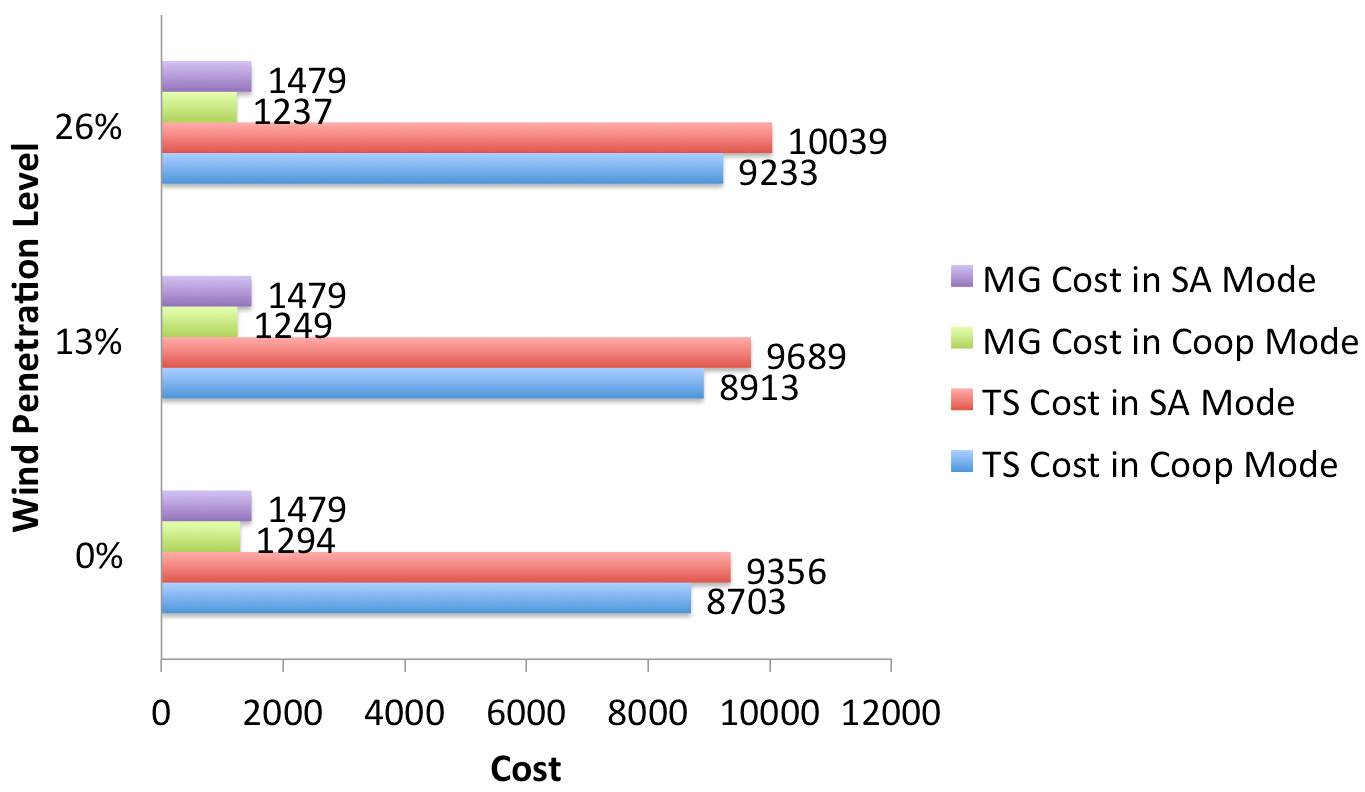
\includegraphics[scale=0.25]{wp1.png}
\caption{TS cost for different WP levels}
\label{pdsize1}
\end{figure}

\begin{figure}[H]
\centering
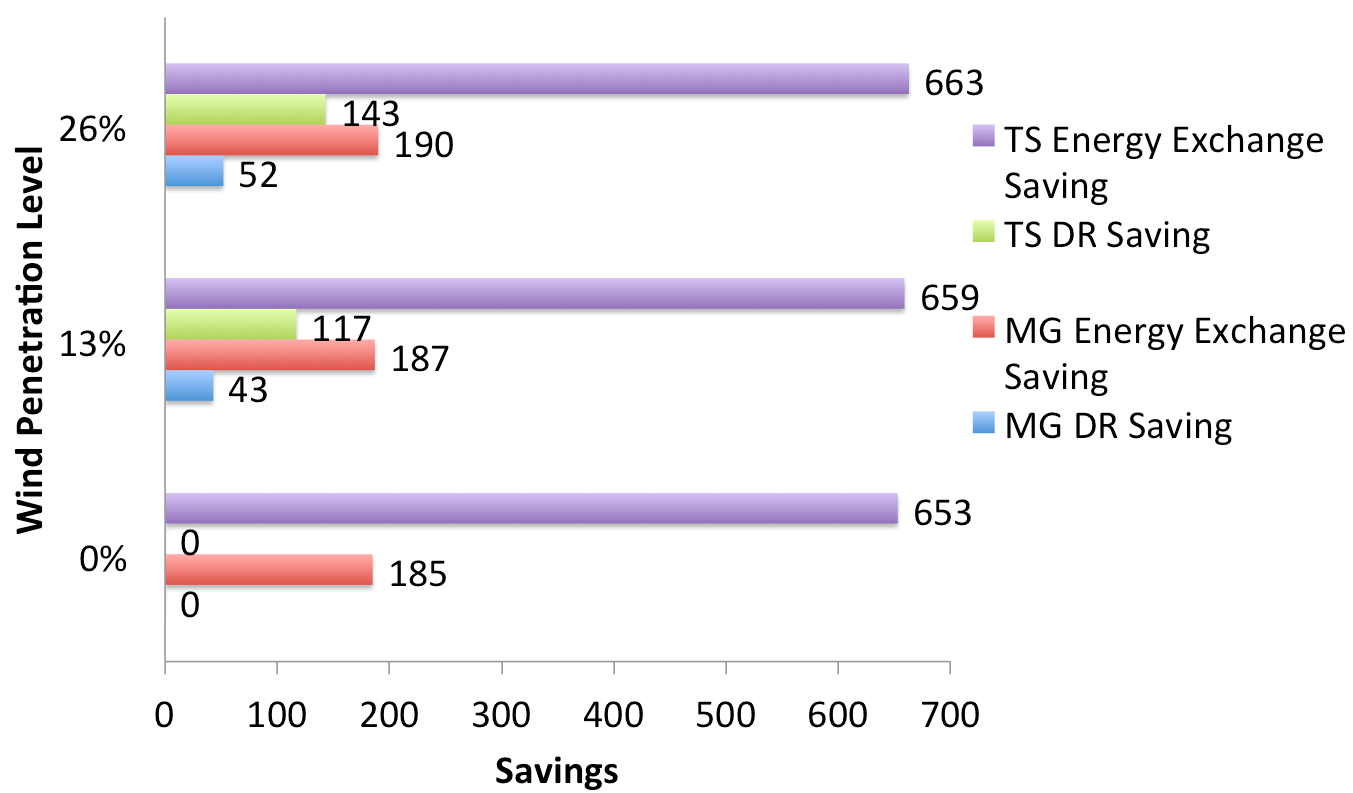
\includegraphics[scale=0.25]{wp2.png}
\caption{TS and MG savings breakdown for different WP levels}
\label{pdsize2}
\end{figure}

From Fig. \ref{pdsize1},  the operational costs of the two systems are smaller in the Coop mode due to the mutual benefits from the energy exchange and DR.   In the SA mode, the MG cost is the same for all three cases as the MG configuration stays the same for all of them. Fig. \ref{pdsize1} shows the break down of the MG and TS savings in terms of DR and energy exchange. When there is no wind, the difference in the operational cost between the operational modes is totally from the energy exchange benefits. As wind penetration increases, the DR savings for the MG and TS increase as more cheaper MG DR is engaged in the ancillary market. The energy exchange saving for the two systems are more or less the same for the three cases as the energy exchange price and quantity (mainly MG import) do not change much. This case study shows that the total saving in the Coop mode with a higher WP is greater for both systems.

\subsubsection{MG size on transmission cost}
The TS is optimized with different sizes of MG connected to bus 5 and the operation cost is reported in Fig. \ref{mgsize}.  For all the cases, the DL level in the MG is 50\%. The wind farm is connected to bus 8, and a fixed 10\% WP is used. 

\begin{figure}[H]
\centering
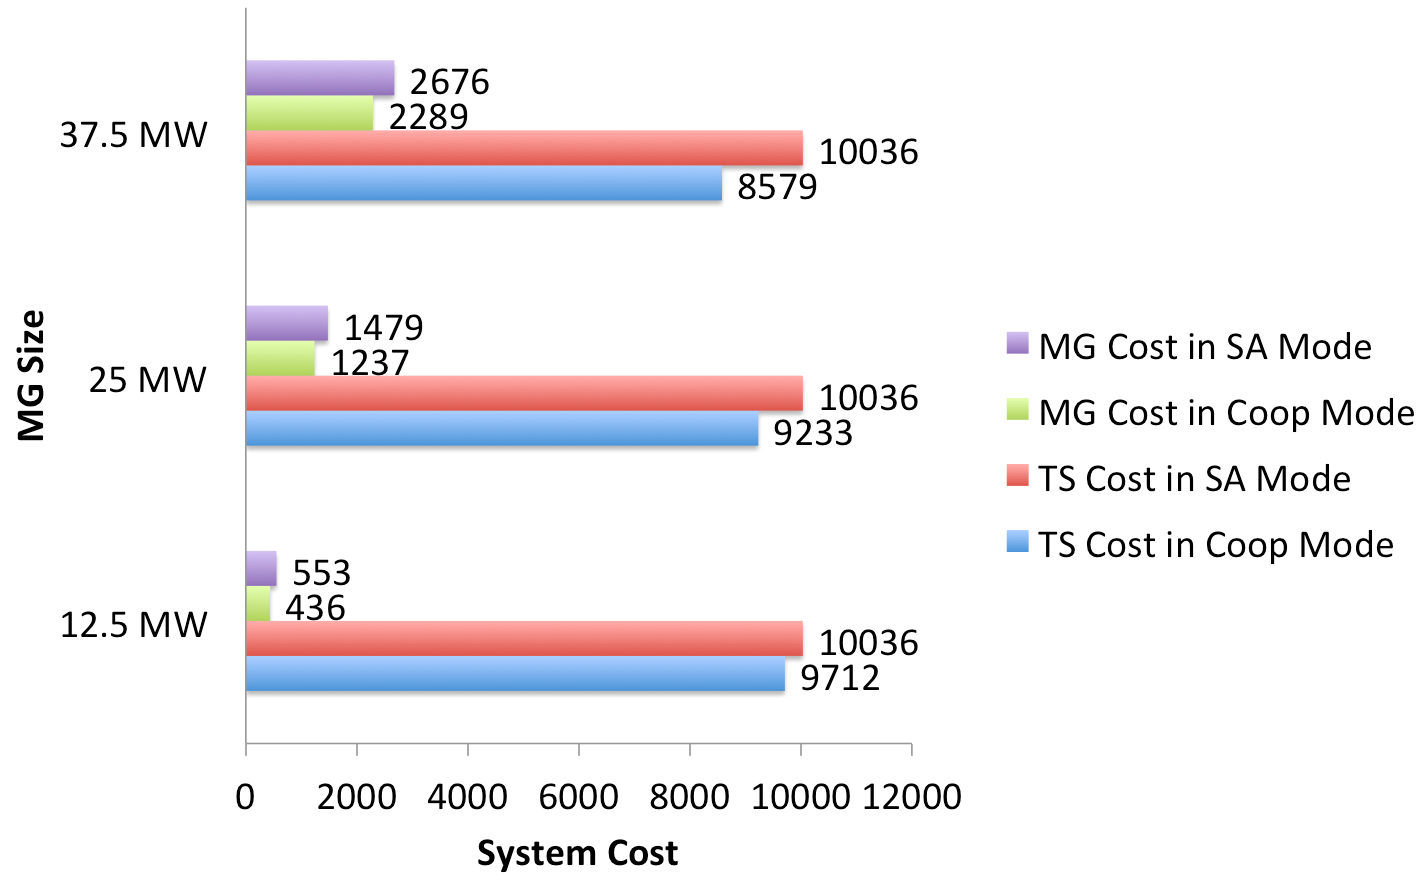
\includegraphics[scale=0.25]{mgsize1.png}
\caption{TS cost for different MG sizes}
\label{mgsize}
\end{figure}

\begin{figure}[H]
\centering
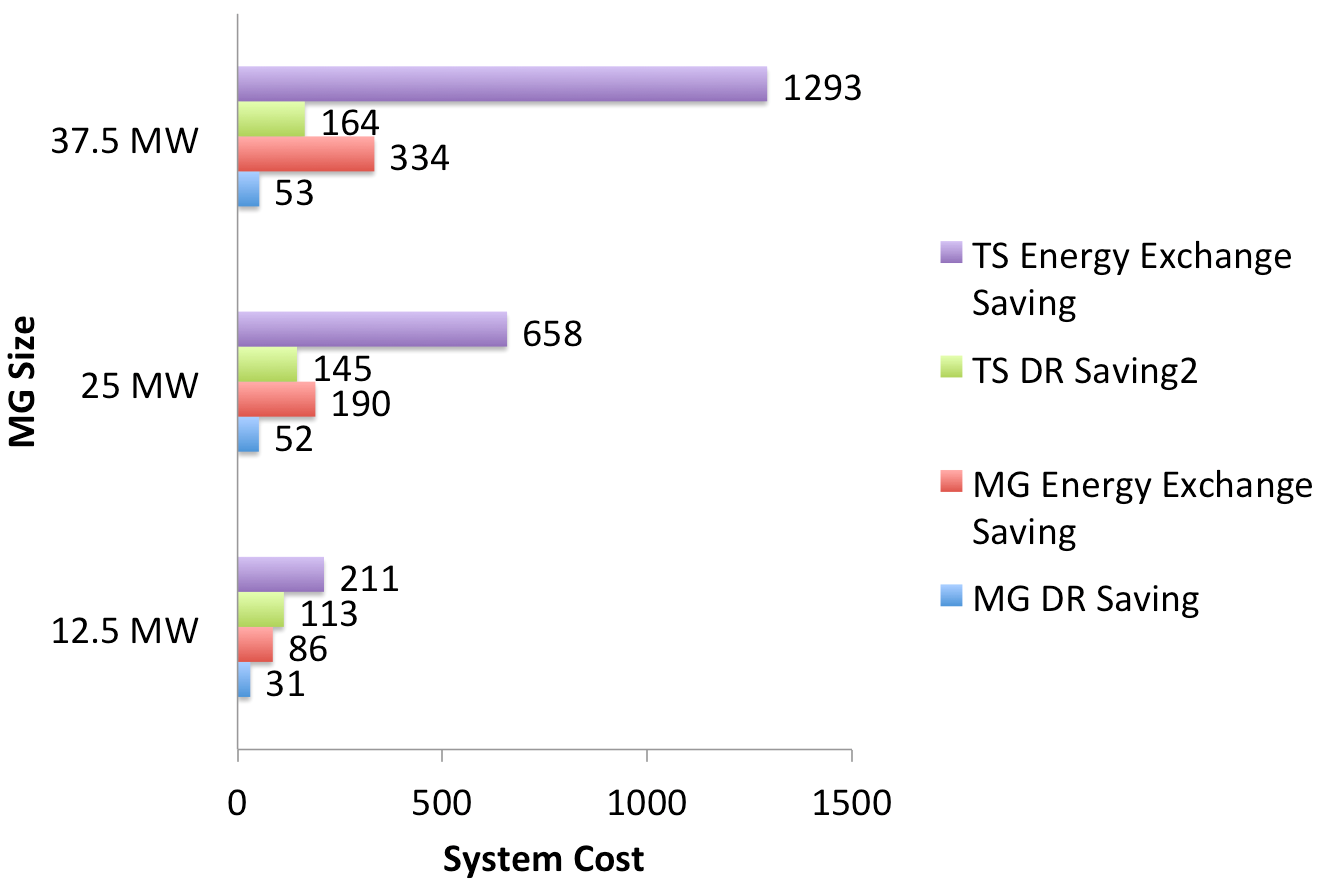
\includegraphics[scale=0.25]{mgsize2.png}
\caption{TS and MG savings breakdown for different MG sizes}
\label{mgsize2}
\end{figure}

From Fig. \ref{mgsize}, it can be seen that in the Co-op mode the cost of the TS decreases with the increase in MG size. That is due to the increased volume of the DR and energy exchange with a larger MG. In addition, the individual system's cost is always smaller in the co-optimization mode compared to the standalone mode as both systems have opportunities to arbitrage in the energy exchange transactions in addition to the benefits from the reserve provision. In the SA mode, the TS cost is the same for all three cases as the TS configuration stays the same for all of them. Fig. \ref{mgsize2} shows the break down of the MG and TS savings in terms of DR and energy exchange. As the MG size increases, the benefits from the energy exchange for both systems increase since the energy exchange volume increases with a larger MG. The DR benefits for both systems also increase as a larger MG could provide more DR service. However the MG DR benefit does not increase much from a 25MW to a 37.5MW MG. That is because the DR price in the latter case is actually lower although the DR provision is greater. This case study shows that the total saving in the Coop mode with a bigger MG is greater for both systems.

\subsubsection{MG DL level on transmission and MG cost}
For the setting of a 25MW MG  and 10\% WP at bus 5 in the TS, the TS and MG operation cost at different levels of MG DL are reported in Fig. \ref{pdsize}.

\begin{figure}[H]
\centering
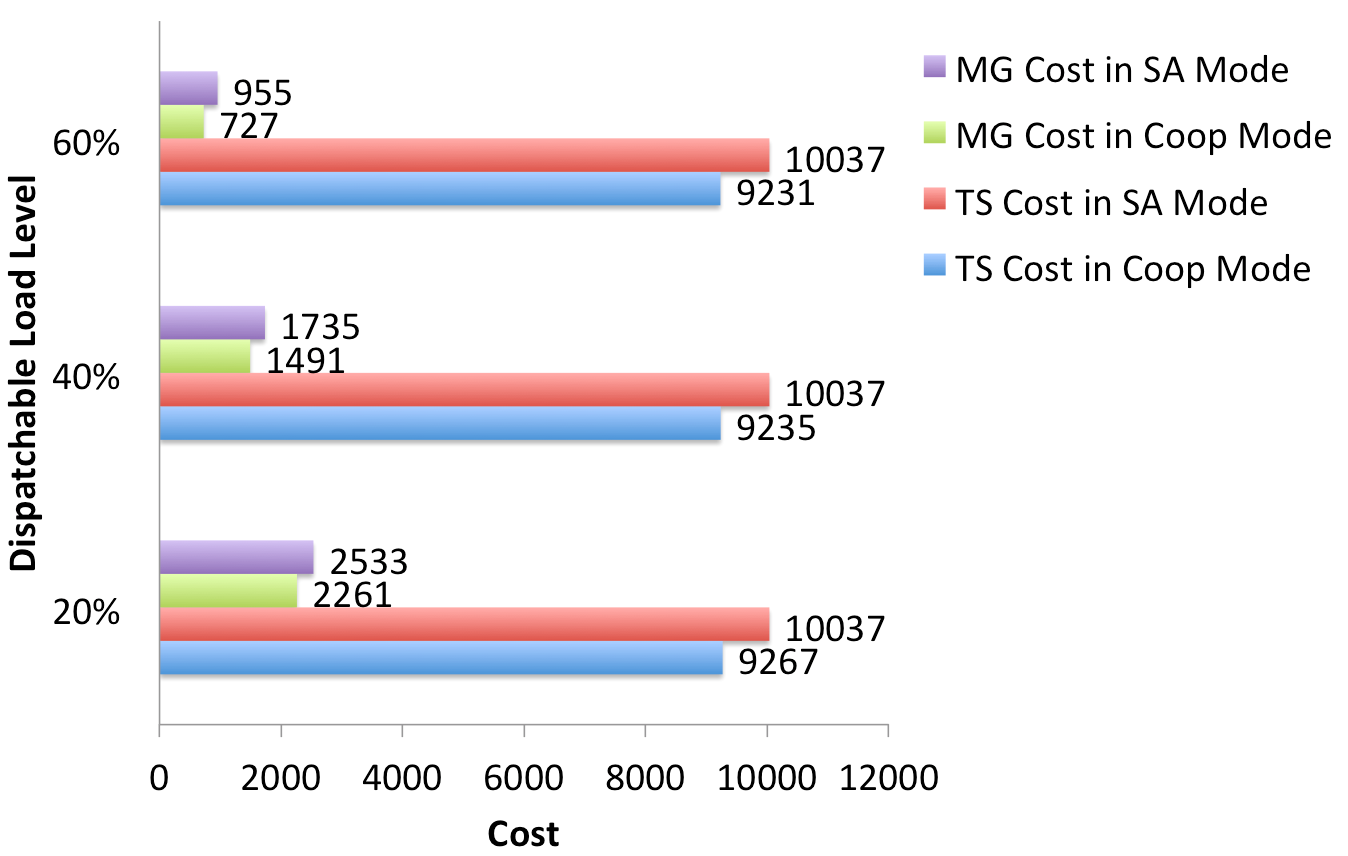
\includegraphics[scale=0.25]{pdsize1.png}
\caption{TS cost for different MG DL levels}
\label{pdsize}
\end{figure}

\begin{figure}[H]
\centering
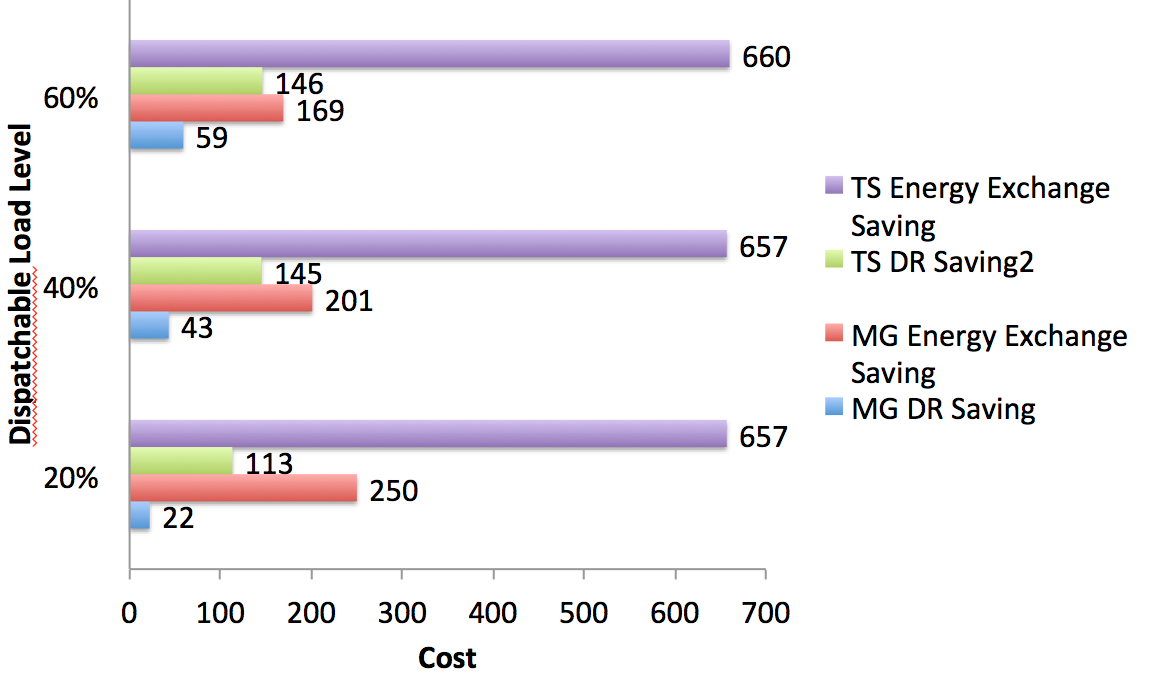
\includegraphics[scale=0.6]{pdsize2.png}
\caption{TS and MG savings breakdown for different MG DL levels}
\label{pdsize2}
\end{figure}

It is shown in Fig.\ref{pdsize} that the TS cost decreases with an increasing DL level as more wind forecast error is accounted by the cheaper MG DR. However that decrease is not significant. In contrast, the MG cost decreases significantly with the increasing DL level as the MG has more DR to sell and more load flexibility. Once again, the Coop framework enables mutual financial benefits from the reserve service and energy exchange and thus reduces the cost of the two systems. The savings breakdown in Fig.\ref{pdsize2} gives further insights about the co-optimization. The energy exchange saving of the TS stays more or less the same for different dispatchable load levels as the net energy exchange quantity with the TS is more or less the same among the three cases. On the contrary, the energy exchange savings for the MG decreases with an increasing dispatchable load level. That is because the cost increasing rate of the MG in the SA mode is great than that in the Coop mode with a decreasing dispatchable load level as the Coop mode enables cost saving from energy exchange. The DR savings for both systems increase with an increasing dispatchable load level as a higher level enables more DR service. However, the DR saving for the TS from 40\% to 60\% DL does not increase much as the marginal cost benefit for that additional DR is very small.

\subsubsection{Wind farm and MG locations on transmission and MG cost}
With 10\% WP, a 25MW MG with 50\% DL system configuration, the location of the wind farm and the MG does not make a difference in terms of the system operation cost as this WP does not cause congestion anywhere in the system. However it is possible that a higher WP at certain buses could cause congestion and significantly increases the system operating cost, which is a well-known fact in the power systems. The way to wisely position the MG to deal with the congestion and reduce the system cost is discussed in \cite{liu2016quantifying}.
